%-----------------------------------------------------------------------------
%
%               Template for sigplanconf LaTeX Class
%
% Name:         sigplanconf-template.tex
%
% Purpose:      A template for sigplanconf.cls, which is a LaTeX 2e class
%               file for SIGPLAN conference proceedings.
%
% Guide:        Refer to "Author's Guide to the ACM SIGPLAN Class,"
%               sigplanconf-guide.pdf
%
% Author:       Paul C. Anagnostopoulos
%               Windfall Software
%               978 371-2316
%               paul@windfall.com
%
% Created:      15 February 2005
%
%-----------------------------------------------------------------------------


\documentclass[preprint]{sigplanconf}

% The following \documentclass options may be useful:

% preprint      Remove this option only once the paper is in final form.
% 10pt          To set in 10-point type instead of 9-point.
% 11pt          To set in 11-point type instead of 9-point.
% numbers       To obtain numeric citation style instead of author/year.

\usepackage{amsmath}
\usepackage{graphicx}
\usepackage{amsthm}
\usepackage{listings}

\newcommand{\cL}{{\cal L}}

\begin{document}

\special{papersize=8.5in,11in}
\setlength{\pdfpageheight}{\paperheight}
\setlength{\pdfpagewidth}{\paperwidth}

\conferenceinfo{CONF 'yy}{Month d--d, 20yy, City, ST, Country}
\copyrightyear{20yy}
\copyrightdata{978-1-nnnn-nnnn-n/yy/mm}
\copyrightdoi{nnnnnnn.nnnnnnn}

% Uncomment the publication rights you want to use.
%\publicationrights{transferred}
%\publicationrights{licensed}     % this is the default
%\publicationrights{author-pays}

% \titlebanner{banner above paper title}        % These are ignored unless
% \preprintfooter{short description of paper}   % 'preprint' option specified.

\title{A New Approach for Parallel Functional Arrays}

\authorinfo{Ananya Kumar}
           {Carnegie Mellon University}
           {ananyak@andrew.cmu.edu}
\authorinfo{Guy Blelloch}
           {Carnegie Mellon University}
           {blelloch@cs.cmu.edu}

\maketitle

\newtheorem{theorem}{Theorem}[section]
\newtheorem{corollary}{Corollary}[theorem]
\newtheorem{lemma}[theorem]{Lemma}
\theoremstyle{definition}
\newtheorem{definition}{Definition}[section]

\begin{abstract}
In this paper we introduce a $O(1)$ wait-free, parallel, functional array, that allows $O(1)$ reads and writes to the most recent version of the array. We describe the cost dynamics and sketch out a provable implementation. We show favorable benchmarks comparing our functional arrays with regular arrays in Java.
\end{abstract}

\category{CR-number}{subcategory}{third-level}

\keywords
array, parallel, cost semantics

\section{Introduction}

Arrays are very important in functional programming languages because they allow work-efficient implementations of algorithms like depth-first search. Accessing old versions of arrays can be useful for efficient checkpointing, logging, and event handling. In this paper we introduce an efficient, parallel, functional array that allows $O(1)$ reads and writes to the most recent version of the array.

\section{Previous Approaches}

Many functional programming languages use monads to build arrays. However, monads do not allow accessing old versions of an array.

Another approach is to use compiler based reference counting. If the number of references to an array is provably one, the compiler allows the array to mutate, otherwise the compiler copies the array before writing to the array. This approach makes it difficult for programmers to reason about the time complexity of array operations because it depends on the compiler. Furthermore, if multiple variables reference the same array, the array is copied even if all writes are to the most recent version. This could make the time complexity of programs significantly higher than they need to be.

A third approach is to use linear types to ensure that programmers can only access and mutate arrays in valid ways. This approach is very difficult to implement in existing programming languages.

O' Neill's functional arrays guarantee $O(1)$ access and insertions when used like an imperative array. However, the arrays use version trees which are inefficient in practice. Additionally, the reads and writes to the most recent version of the array might take $O(\log{n})$ work if the array is not used like an imperative array.

Chuang's approach supports $O(1)$ accesses and insertions to the most recent version of arrays, however accessing old versions of the array takes $O(n)$ work which is often impractical.

None of the existing approaches support concurrent operations on arrays. O' Neill suggests having a lock for each element of the array. However, when many threads contend for the same element, this would serialize accesses and make accesses not $O(1)$. Additionally, per-element locks add significant memory overhead. Separation logic could be used to parallelize divide and conquer algorithms on arrays however they would severely restrict the way functional arrays can be used.

\section{Dynamics}

We use a standard applicative-order language defined as follows:
$$L = x \; | \; c  \; | \; \lambda x.e \; | \; f \; x \; | \; e_1 || e_2 \; | \; \text{if } e_1 \text{ then } e_2 \text{ else } e_3$$

$L$ contains the usual arithmetic types, such as the natural numbers, and numerical operations such as sums and products. Dynamics for function application and fork-join are given as examples.
$$\frac{e_1 \Downarrow v_1 \;\;\; e_2 \Downarrow v_2}{e_1 || e_2 \Downarrow (v_1, v_2)} \text{ (fork-join)}$$
$$\frac{f \Downarrow \lambda x . e \;\;\; y \Downarrow v}{f \; y \Downarrow [v/x]e} \text{ (function-app)}$$

The language also includes 3 functions for working with arrays: tabulate, get, and set. The dynamics for tabulate is given below:
$$\frac{f(1) \Downarrow v_1, ..., f(n) \Downarrow v_n}{\text{tabulate} \; f \; n \Downarrow [1 \mapsto v_1, ..., n \mapsto v_n]}$$

The dynamics for the other two array functions are standard.

\section{Approach}

An array $A$ is NEW if the set function has not been called with $A$ as an argument, otherwise $A$ is OLD. While the dynamics of our arrays are functional, the costs are different for OLD and NEW arrays. 

\begin{figure}[!ht]
\centering
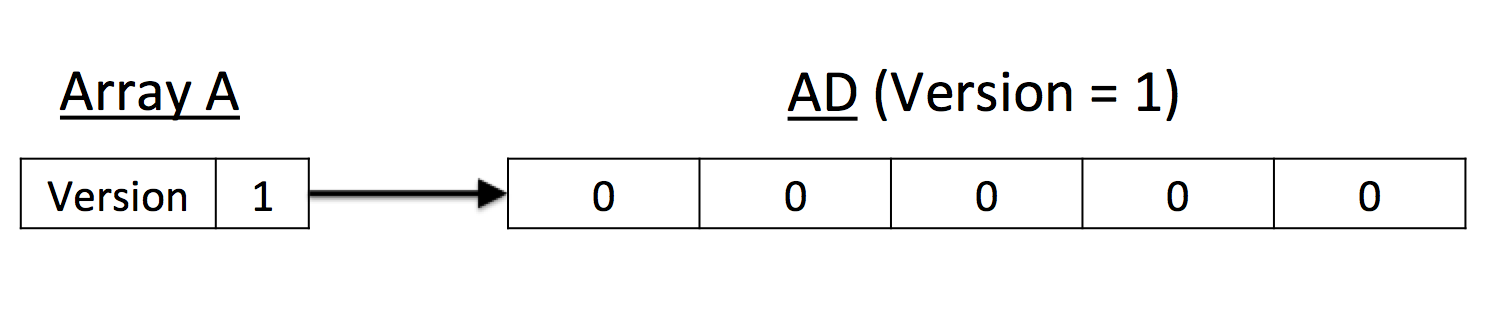
\includegraphics[scale=0.3]{new_array_A}
\nocaptionrule \caption{New functional array filled with 0s}
\label{fig:new_array_A}
\end{figure}

Suppose that $A$ is a NEW functional array  (see figure \ref{fig:new_array_A}). $A$ has a version number $V$, and a pointer to an ArrayData object $AD$. $AD$ keeps a regular (mutable) array of values, which corresponds to the values in $A$. $AD$ has a version number, which is the same as $A'$s ($V$) to indicate that $A$ is NEW. For each element of the array in $AD$, keep a log of values that used to be at that index. The logs are initially empty.

Get on NEW arrays: to get the $i^{\text{th}}$ element in $A$, simply access array[i] in $AD$.

\begin{figure}[!ht]
\centering
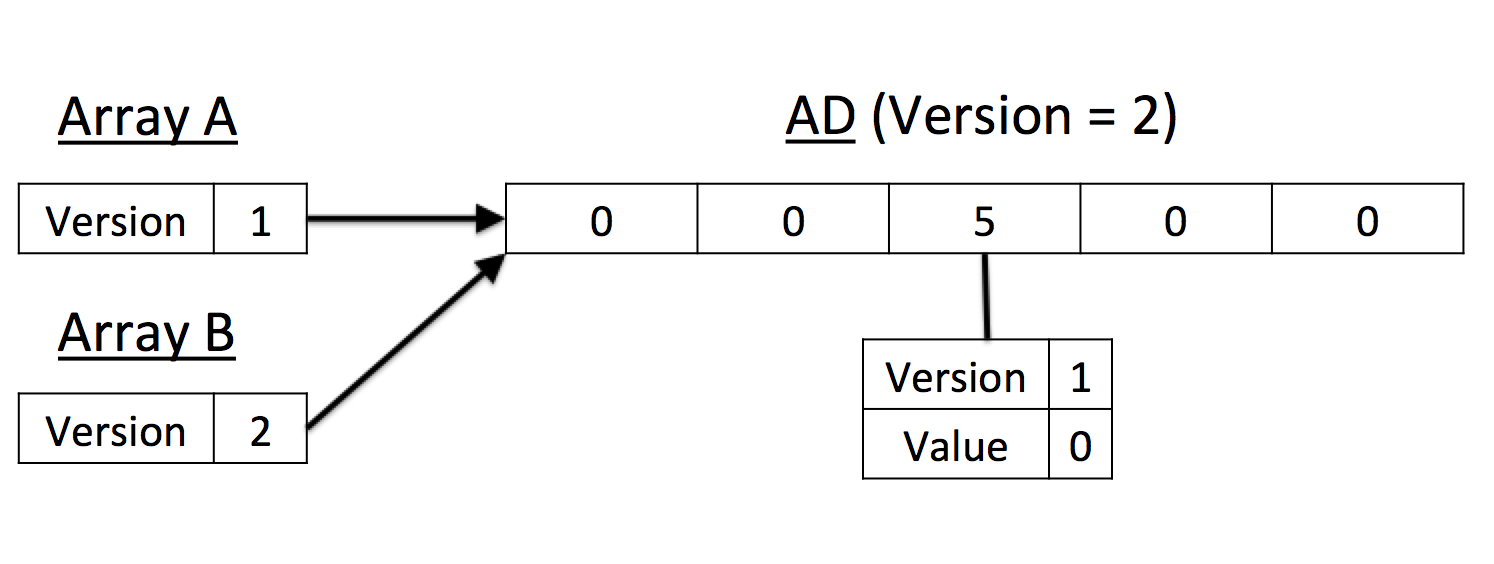
\includegraphics[scale=0.3]{set_A_return_B}
\nocaptionrule \caption{$B = set(A, 3, 5)$ changes the array in $AD$ and adds a log entry.}
\label{fig:set_A_return_B}
\end{figure}

Set on NEW arrays: Suppose that $A[i]$ is $v_{old}$ and we want to do $B = set(A, i, v_{new})$ (see figure \ref{fig:set_A_return_B}). Add an entry $(V, v_{old})$ to the log at index $i$, expressing that $A[i]$ was $v_{old}$ at version $V$. Increment the version of $AD$ to $V+1$. Set $array[i]$ in $AD$ to $v_{new}$. Create a new functional array $B$, with version $V+1$, which points to $AD$. Notice that both $A$ and $B$ point to $AD$. However, the version of $A$ is $V$ and the version of $AD$ is $V+1$, which indicates that $A$ is OLD. The version of $B$ is $V+1$ which indicates that $B$ is NEW.

Get on OLD array: Suppose we do $get(A, i)$ where $A$ is OLD and has version $V$. We binary search the log at index $i$ to find what value was stored in the array at version $V$.

\begin{figure}[!ht]
\centering
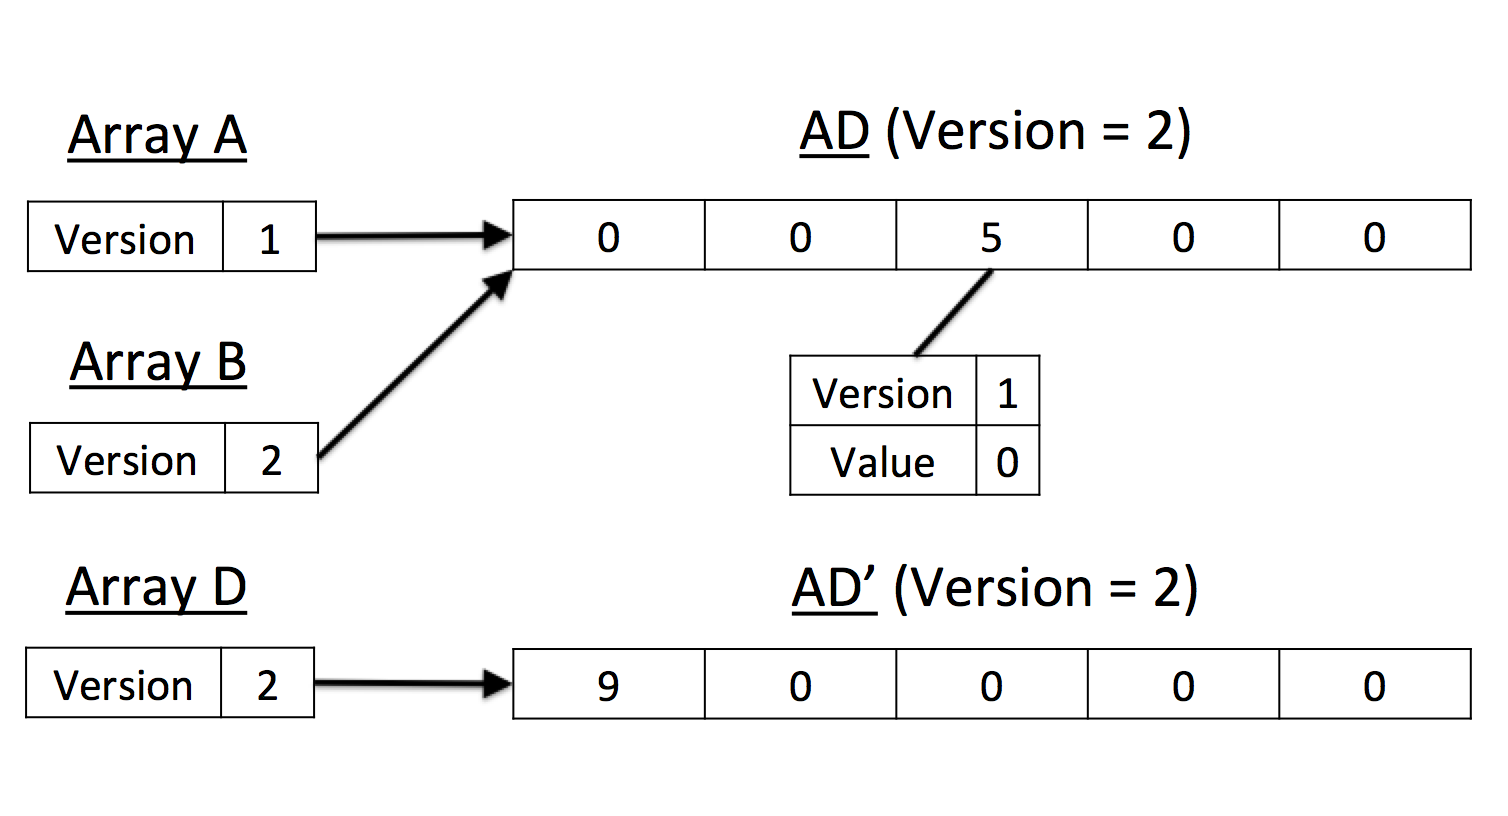
\includegraphics[scale=0.3]{set_old_array}
\nocaptionrule \caption{$D = set(A, 1, 9)$ copies $AD$ because $A$ is OLD}
\label{fig:set_old_array}
\end{figure}

Suppose we do $D = set(A, i,v)$ where $A$ is old (see figure \ref{fig:set_old_array}). Create a new ArrayData object $AD'$ (with a new array). Copy the values from the array in $AD$ to the array in $AD'$, and then set $array[i]$ to $v$ in $AD'$.

The logs are stored in a doubling array which doubles in size when full. This guarantees amortized $O(1)$ insertion of a log entry, and allows us to binary search with $O(\log{m})$ work, where $m$ is the number of log entries.

Suppose that the size of the array is $n$. Every $n$ times an ArrayData object is modified, we create a new ArrayData object, and copy the values over to the new ArrayData object. This ensures that $m \leq n$ i.e. we don't have too many log entries in an ArrayData object. Copying is amortized $O(1)$.

It follows that in the RAM model the work of set and get is $O(1)$ for a NEW array. Get in an OLD array involves a binary search and has work $O(\log{n})$. Set in an OLD array involves copying the array, and has work $O(n)$.

\section{Cost Dynamics}

Arrays are represented by $(l, D)$ where $l$ is a label that uniquely identifies the array, and $D$ contains the values in the array. $D[i]$ is the $i^{\text{th}}$ value in the array. If the set method has been applied on an array, the array is OLD (represented by $-$), otherwise the array is NEW (represented by $+$). 

Array methods have different costs depending on whether the array is NEW or OLD. Let $C(l)$ be the number of get operations applied on array $A = (l, D)$ that had $O(1)$ work. We thread a store $\delta$ through each operation. $\delta$ maps array labels $l$ to $(+/-, c)$, where $c = C(l)$.

Our cost dynamics are defined by the following judgement, where $\delta$ is the store, $f$ is the array function being applied, $\delta'$ is the new store, $v$ is the value returned by applying $f$ on $args$, $w$ is the work, and $s$ is the span.
$$\delta; f \; args \Downarrow \delta'; v; w; s$$
The cost dynamics for the methods on a functional array of size $n$ are:
$$\frac{l = \text{new label} \;\;\; f(1) \Downarrow v_1; w_1; s_1; ... f(n) \Downarrow v_{n}; w_{n}; s_{n}}{\delta; \text{tabulate } f \; n \Downarrow \delta[l \mapsto (+, 0)]; (l, \bigcup_{i=1}^n [i \mapsto v_i]); 1+\sum w_i; 1+\max s_i}$$
$$\frac{\delta[l \mapsto (+, c)] \;\;\; A = (l,D) \;\;\; l' = \text{new label}}{\delta; \text{set} \; A \; i \; v \Downarrow \delta[l \mapsto (-, c), l' \mapsto (+, 0)]; (l', D[i \mapsto v]); 1; 1} \text{  (set-new)}$$
$$\frac{\delta[l \mapsto (-, c)] \;\;\; A = (l,D) \;\;\;  l' = \text{new label}}{\delta; \text{set} \; A \; i \; v \Downarrow \delta[l \mapsto (-, c), l' \mapsto (+, 0)]; (l', D[i \mapsto v]); n; 1} \text{  (set-old)}$$
$$\frac{\delta[l \mapsto (+, c)] \;\;\; A = (l,D)}{\delta; \text{get} \; A \; i \Downarrow \delta[l \mapsto (+, c+1)]; D[i]; 1; 1} \text{  (get-new)}$$
$$\frac{\delta[l \mapsto (-, c)] \;\;\; A = (l,D)}{\delta; \text{get} \; A \; i \Downarrow \delta; D[i]; \log{n}; 1} \text{  (get-old)}$$

The fork-join cost semantics are the most interesting. We give the cost dynamic using 2 helper functions. Let $L(\delta)$ denote the set of labels in the store $\delta$. Let $f(n)$ be the cost of calling get on an OLD array and $g(n)$ be the cost of calling set on an OLD array.
\begin{align*}
\text{def NEW}&\text{-MAP: }L(\delta_1) \cup L(\delta_2) \to (+/-, \text{int}) = \\
\text{Case } &\delta[l \mapsto (-,c)]: (-, c)  \\
\text{Case } &\delta[l \mapsto (+,c)]:  \\
&\text{Case } \delta_1[l \mapsto (+,c+x)], \delta_2[l \mapsto (+,c+y)]: (+, c+x+y) \\
&\text{Case } \delta_1[l \mapsto (+,c+x)], \delta_2[l \mapsto (-,c+y)]: (-, c+y) \\
&\text{Case } \delta_1[l \mapsto (-,c+x)], \delta_2[l \mapsto (+,c+y)]: (-, c+x) \\
&\text{Case } \delta_1[l \mapsto (-,c+x)], \delta_2[l \mapsto (-,c+y)]: (-, c) \\
\text{Else: } & \\
&\text{Case } \delta_1[l \mapsto (s,c)]: (s,c) \\
&\text{Case } \delta_2[l \mapsto (s,c)]: (s,c) \\
\text{def EXT}&\text{RA-WORK: }L(\delta_1) \cup L(\delta_2) \to int = \\
\text{Case } &\delta[l \mapsto (+,c)]:  \\
&\text{Case } \delta_1[l \mapsto (+,c+x)], \delta_2[l \mapsto (+,c+y)]: 0 \\
&\text{Case } \delta_1[l \mapsto (+,c+x)], \delta_2[l \mapsto (-,c+y)]: x f(n) \\
&\text{Case } \delta_1[l \mapsto (-,c+x)], \delta_2[l \mapsto (+,c+y)]: y f(n) \\
&\text{Case } \delta_1[l \mapsto (-,c+x)], \delta_2[l \mapsto (-,c+y)]: (x+y)f(n) + g(n) \\
\text{Else: } & 0
\end{align*}											
$$\delta' = \bigcup_{l \in L(\delta_1) \cup L(\delta_2)} \text{NEW-MAP} (l)$$
$$w' = \sum_{l \in L(\delta_1) \cup L(\delta_2)} \text{EXTRA-WORK} (l)$$
Then, the fork-join cost semantics are:
$$\delta; e_1 || e_2 \Downarrow \delta'; (v_1, v_2); 1 + w_1 + w_2 + w'; 1 + \max(s_1, s_2)$$

\section{Concurrent Implementation}

We implement the functional array functions using an imperative target language.

\subsection{Concurrency Model}

We assume a sequential consistency model of concurrency. That is, when analyzing the effects of a program, we assume that at each time step exactly one pending instruction is executed. Consider the execution of a program $P$. We label the time steps in the execution from 1 to $t$. 

\begin{definition}
Consider an object $A$. Suppose that the program invokes methods $M_1$, $M_2$, ..., $M_n$ on $A$. Consider arbitrary $i$, and suppose that the instructions in $M_i$ were executed at times $s_1$, $s_2$, ..., $s_m$. We say that $A$ is \emph{linearizable} if the effect of the program is as if $M_i$ executed atomically at some time $s_j$, and this holds for all $M_i$.
\end{definition}

\begin{definition}
Suppose that first instruction in function call $f$ was executed at time $s_1$ and the last instruction at time $e_1$. Suppose that first instruction in function call $g$ was executed at time $s_2$ and the last instruction at time $e_2$. We say the function calls do not \emph{overlap} if the intervals $[s_1, e_1]$ and $[s_2, e_2]$ do not overlap.
\end{definition} 

Our programs have access to the link load store conditional (LLSC) function. LLSC takes an (address, old value, new value) tuple as argument. LLSC first checks that the value at address is the same as old value, if it is different then LLSC returns false. Otherwise LLSC atomically stores new value at address and returns true, however if the value at address was modified between the load and store, LLSC returns false.

\subsection{Push Arrays}

We use an auxiliary data structure, \emph{PushArrays}, to store log entries. PushArrays are initially empty and support 3 methods. Suppose we have a PushArray $A$. $A.push(e)$ inserts entry $e$, $A.size()$ returns the number of entries inserted, $A.get(i)$ returns the $i^{\text{th}}$ entry inserted. Note that $get$ is only defined between indices 0 and $A.size()-1$. All operations are amortized $O(1)$.

PushArrays can be used semi-concurrently. At most one thread can execute $push$ at any time, but multiple threads can call $size$ and $get$. In a PushArray $A$, $A.size$ stores the number of entries and $A.data$ references an array that stores the actual entries. Pseudocode for $A.push(e)$ is shown below.

\begin{lstlisting}[language=Java]
if (isFull(A.data)) {
  newData = new Array(A.data.capacity * 2);
  copyValues(from = A.data, to = newData);
  A.data = newData;
}
A.data[A.size] = e;
A.size += 1;
\end{lstlisting}

\begin{theorem}
Given that different calls to push (on the same PushArray) do not overlap, PushArrays are linearizable.
\end{theorem}

\begin{proof}
The linearization point of $push$ is $A.size$ $+=$ $1$, and the linearization point of the other methods is their single instruction. In push, expanding the capacity of $A.data$ when it is full does not interfere with accessing $A.data$ because we copy values to the new array before pointing $A.data$ to the new array. The effects of adding $e$ are only observable after we increase $size$, since, by the specification of PushArrays, the result of calling $A.get(i)$ where $i \geq A.size()$ is not defined.
\end{proof}

\subsection{Functional Array Implementation}

Suppose we have a FunctionalArray $A$. $A$ points to an ArrayData object which is referenced by $A.data$. The (imperative) array in $A.data$ is referenced by $A.data.values$, and the log entries corresponding to the $i^{\text{th}}$ index are stored in a PushArray $A.data.undo\_lists[i]$. We first explain the implementation of $A.set(pos, val)$.

We use a link load store conditional to ensure that only 1 thread can modify an ArrayData object at any time. If $m$ threads try to modify $A.data$, then $m-1$ threads will fail the LLSC (returning false). Instead of modifying $A.data$, these threads will create a new ArrayData object, and will copy over values from $A.data$, as shown below.

\begin{lstlisting}[language=Java]
FunctionalArray newA;
newA.version = A.version + 1;
if (!LLSC(&A.data.version, A.version, 
	newA.version)) {
  // Create a new ArrayData object AD
  // Copy A.data.values to AD.values
  AD.values[pos] = val;
  newA.data = AD;
  return newA;
}
\end{lstlisting}

One of the threads trying to modify the ArrayData object will get past the LLSC, will insert a log entry and then modify $A.data.values$. The ordering of inserting a log entry and modifying $A.data.values$ matters in the proof of get The pseudocode for this step is shown below.

\begin{lstlisting}[language=Java]
newA.data = A.data;
old_value = newA.data.values[pos];
undo_list = newA.data.undo_lists[pos];
undo_list.push((A.version, old_value));
newA.data.values[pos] = val;
return newA;
\end{lstlisting}

Next we explain the implementation of $A.get(pos)$.

\begin{lstlisting}[language=Java]
guess_val = A.data.values[pos];
if (A.version == A.data.version) {
  return guess_val;
}

undo_list = this.data.undo_lists[pos];
if (undo_list.size() == 0) {
  return guess_val;
}

upper = undo_list.size() - 1;
if (undo_list[upper].version < A.version) {
  return guess_val;
}
\end{lstlisting}

The last step is to binary search $undo\_list$, between the indices 0 and $upper$ (inclusive of 0 and upper). We find the log entry $L$ with the smallest version $X$ such that $A.version \leq X$. We return $L.value$.

The implementation of tabulate is straightforward - just allocate a new array and fill the array with the required values.

\subsection{Proof of Correctness}

\begin{theorem}
Functional Arrays are linearizable.
\end{theorem}

\begin{proof}
We can choose any instruction in the execution of get as the linearization point - we arbitrarily choose the first instruction. The linearization point of set is the LLSC. Any instruction in tabulate can be its linearization point - we omit discussion of tabulate because the details are uninteresting.

First, we prove the linearization point of get. (fill this out)

Next, we prove the linearization point of set. (fill this out)

\end{proof}

In a previous section, we gave the evaluational (big step) dynamics of functional arrays. Alternatively, we could give the non-deterministic structural (little step) dynamics which describes the steps in the execution of a program in the source language. At each fork-join, if both sides of the fork can take a step, we could take a step on either side.

\begin{theorem}
Suppose that the execution of a program in the target language has a certain linear order of function calls $M_1$, $M_2$, ... $M_n$. Then there exists a (little step) transition sequence in the source language where the functions are called in the same order.
\end{theorem}

\begin{proof}
Fill this out. Use induction.
\end{proof}

\begin{theorem}
Suppose that the execution of a program in the target language has a certain linear order of function calls $M_1$, $M_2$, ... $M_n$ and consider a little step transition sequence in the source language where the functions are called in the same order $F_1$, $F_2$, ..., $F_n$. For any $F_i$, if $F_i$ is a get, then the value returned by $M_i$ and $F_i$ are the same.
\end{theorem}

\begin{proof}
Note that this is the sequential proof of correctness. Consider arbitrary $i$ and suppose that functional calls $F_j$ for $j \leq i$ have executed in the source language and function calls $M_j$ for $j \leq i$ have executed in the target language. Consider an arbitrary array $A'$ in the source language and corresponding array $A$ in the target language. We claim that the following data structure invariant holds:

Consider arbitrary index $i$ and suppose that $A'[i]$ has value $val$. Suppose that $A$ has version $V$ and is pointing to an ArrayData object $AD$. Either there exists some version in $AD.logs[i]$ which is greater than $V$ in which case there exists a log entry $(v', val)$ where $v'$ is the smallest version in $AD.logs[i]$ that is $\geq V$. Or $AD.values[i]$ is val.

The data structure invariant can be proved by induction, we present a sketch. The base case is trivial. In the inductive case, get does not mutate any array. When we do a set operation, the invariant holds for the new array because we modify the value in its ArrayData object. It holds for other arrays in the target language that might have been mutated because we insert log entries.

Given that the data structure invariant holds, it is easy to see that any call to get returns the same value in the source and target language (maybe we need a little more detail here?).
\end{proof}

\begin{theorem}
The non-deterministic structural dynamics and the evaluational dynamics produce the same result in the source language.
\end{theorem}

\begin{proof}
This is a standard programming languages proof so we omit the proof.
\end{proof}

We have shown that there exists a transition sequence that our implementation correctly simulates, and that all transition sequences are equivalent to the evaluational dynamics, so our implementation correctly simulates the evaluational dynamics.

\section{Correctness}

\section{Machine Model}

Our target language is a Java-like language augmented with tabulate, fork-join, lambda functions, and link load store conditional (LLSC). Fork-join spawns two threads, one thread executing each sub-expression. Link load store conditional (LLSC) takes an (address, old value, new value) tuple as argument. LLSC first checks that the value at address is the same as old value, if it is different then LLSC returns false. Otherwise LLSC atomically stores new value at address and returns true, however if the value at address was modified between the load and store, LLSC returns false.

Our target language is run on a P processor machine. In a single time step the machine takes at most P runnable instructions and executes them.  The effect of executing the ($\leq P$) instructions in a time step is the same as some (arbitrary) sequential ordering of the instructions. We assume that the machine does not reorder instructions in the target language. In reality, languages like Java have very relaxed consistency models, and we deal with this in our real implementation using memory fences.

The link load store conditional architecture deserves special mention. Call an LLSC operation pending if the load operation has completed but the store operation has not. Multiple threads can load the value at a particular address and compare it with old value in a single time step. Only a single store operation to a particular address can be executed at a time step. However, after the store operation, in each time step the bus arbiter notifies all pending LLSC operations to the same memory address that they have failed. This assumption is reasonable because all LLSC instructions are typically processed by the bus arbiter, so the bus arbiter can keep track of pending LLSC instructions to each memory address.


% We recommend abbrvnat bibliography style.

\bibliographystyle{abbrvnat}

% The bibliography should be embedded for final submission.

\bibliography{references}

\end{document}
